\documentclass[border=10pt]{standalone}
\usepackage{graphicx} % for including graphics
\usepackage{tikz}
\usepackage{minted}
\usepackage[urlcolor=blue]{hyperref}
\usepackage{multirow}
\usepackage{adjustbox}

\usetikzlibrary{calc,matrix,decorations.markings,decorations.pathreplacing,fit}

\definecolor{bg-terminal}{HTML}{666666}
\definecolor{border-terminal}{HTML}{efefef}
\definecolor{bg-python}{HTML}{244c6f}
\definecolor{border-python}{HTML}{eff7ff}
\definecolor{bg-restapi}{HTML}{4d5a31}
\definecolor{border-restapi}{HTML}{e4ffa7}
\definecolor{bg-dataset}{HTML}{95319b}
\definecolor{border-dataset}{HTML}{f5ecff}

\definecolor{bg-descriptive}{HTML}{f1e8fa}
\definecolor{fg-descriptive}{HTML}{4b128d}
\definecolor{bg-administrative}{HTML}{faebe3}
\definecolor{fg-administrative}{HTML}{ce561a}
\definecolor{bg-structural}{HTML}{f1faec}
\definecolor{fg-structural}{HTML}{44a315}

\definecolor{bg-tags}{HTML}{f5ecff}
\definecolor{bg-annotations}{HTML}{f5ecff}
\definecolor{bg-readme}{HTML}{f5ecff}
\definecolor{bg-admin}{HTML}{ffefe7}
\definecolor{bg-manifest}{HTML}{f5fff0}
\definecolor{bg-data}{HTML}{f5fff0}

\definecolor{http-get-dark}{HTML}{61affe}
\definecolor{http-get-light}{HTML}{eff7ff}
\definecolor{http-put-dark}{HTML}{fca130}
\definecolor{http-put-light}{HTML}{fff5ea}
\definecolor{http-post-dark}{HTML}{49cc90}
\definecolor{http-post-light}{HTML}{ecfaf4}
\definecolor{http-delete-dark}{HTML}{f93e3e}
\definecolor{http-delete-light}{HTML}{feebeb}

\definecolor{tag}{HTML}{95319b}

% Define box and box title style
\tikzstyle{tag} = [
	draw=tag, 
	fill=tag, 
	text=white, 
	rectangle, 
	rounded corners, 
	minimum height=1.4\baselineskip
]

\tikzstyle{http-method} = [
	text=white, 
	font=\bfseries,
	rectangle, 
	rounded corners, 
	minimum height=1.4\baselineskip, 
	minimum width=1.8cm
]

\tikzstyle{http-method-frame} = [
	text=black, 
	rectangle, 
	rounded corners, 
	minimum height=1.8\baselineskip, 
	minimum width=8cm
]

\tikzstyle{http-route} = [
	text=black, font=\ttfamily
]

\tikzset{ 
  dataset-table/.style={
    matrix of nodes,
    row sep=-\pgflinewidth,
    column sep=-\pgflinewidth,
    nodes={rectangle,align=left},
    text depth=1.25ex,
    text height=2.5ex,
    nodes in empty cells,
    column 1/.style={
	  nodes={
	  	text width=10cm
	  }
	},
	column 2/.style={
	  nodes={
	  	text width=0.5cm
	  }
	},
	row 1/.style={
        nodes={
           minimum height=4\baselineskip
        }
    },
    row 2/.style={
        nodes={
           minimum height=5\baselineskip
        }
    },
    row 3/.style={
        nodes={
           minimum height=14.5\baselineskip
        }
    },
    row 4/.style={
        nodes={
           minimum height=10.0\baselineskip
        }
    },
    row 5/.style={
        nodes={
           minimum height=13.5\baselineskip
        }
    },
    row 6/.style={
        nodes={
           minimum height=5.5\baselineskip
        }
    }
  }
}

\tikzset{ 
  terminal-table/.style={
    matrix of nodes,
    row sep=-\pgflinewidth,
    column sep=-\pgflinewidth,
    nodes={rectangle,align=left},
    text depth=1.25ex,
    text height=2.5ex,
    nodes in empty cells,
    column 1/.style={
	  nodes={
	  	text width=10cm
	  }
	},
	column 2/.style={
	  nodes={
	  	text width=0.5cm
	  }
	},
	row 1/.style={
        nodes={
           minimum height=5\baselineskip
        }
    },
    row 2/.style={
        nodes={
           minimum height=5\baselineskip
        }
    },
    row 3/.style={
        nodes={
           minimum height=13.5\baselineskip
        }
    },
    row 4/.style={
        nodes={
           minimum height=8.5\baselineskip
        }
    },
    row 5/.style={
        nodes={
           minimum height=6\baselineskip
        }
    },
    row 6/.style={
        nodes={
           minimum height=14.5\baselineskip
        }
    }
  }
}

\tikzset{ 
  python-table/.style={
    matrix of nodes,
    row sep=-\pgflinewidth,
    column sep=-\pgflinewidth,
    nodes={rectangle,align=left},
    text depth=1.25ex,
    text height=2.5ex,
    nodes in empty cells,
    column 1/.style={
	  nodes={
	  	text width=10cm
	  }
	},
	column 2/.style={
	  nodes={
	  	text width=0.5cm
	  }
	},
	row 1/.style={
        nodes={
           minimum height=7\baselineskip
        }
    },
    row 2/.style={
        nodes={
           minimum height=5.5\baselineskip
        }
    },
    row 3/.style={
        nodes={
           minimum height=8\baselineskip
        }
    },
    row 4/.style={
        nodes={
           minimum height=5.5\baselineskip
        }
    },
    row 5/.style={
        nodes={
           minimum height=12\baselineskip
        }
    },
    row 6/.style={
        nodes={
           minimum height=14.5\baselineskip
        }
    }
  }
}

\tikzset{ 
  restapi-table/.style={
    matrix of nodes,
    row sep=-\pgflinewidth,
    column sep=-\pgflinewidth,
    nodes={rectangle,align=left},
    text depth=1.25ex,
    text height=2.5ex,
    nodes in empty cells,
    column 1/.style={
	  nodes={
	  	text width=10cm
	  }
	},
	column 2/.style={
	  nodes={
	  	text width=0.5cm
	  }
	},
	row 1/.style={
        nodes={
           minimum height=6.5\baselineskip
        }
    },
    row 2/.style={
        nodes={
           minimum height=4.5\baselineskip
        }
    },
    row 3/.style={
        nodes={
           minimum height=4.5\baselineskip
        }
    },
    row 4/.style={
        nodes={
           minimum height=19.0\baselineskip
        }
    },
    row 5/.style={
        nodes={
           minimum height=15.5\baselineskip
        }
    },
    row 6/.style={
        nodes={
           minimum height=2.5\baselineskip
        }
    }
  }
}

\setminted{
   baselinestretch=1.1,
   bgcolor=white,
   fontsize=\footnotesize
}
       
\def\exampleindent{3em}

\renewcommand*{\familydefault}{\sfdefault}
\newcommand{\cbox}[1]{\parbox[t]{5cm}{#1}}
\newcommand{\lbox}[1]{\parbox[t]{10cm}{#1}}

\begin{document}
%
% We need layers to draw the block diagram
\pgfdeclarelayer{background}
\pgfdeclarelayer{foreground}
\pgfsetlayers{background,main,foreground}
%
\trimbox{0cm 0cm 4cm 0cm}{
\begin{tikzpicture}
  \begin{scope}[shift={(0.4cm,0)}]
  \matrix (mat) [dataset-table] {
    |[fill=bg-tags]| & |[fill=bg-descriptive]| \\
    |[fill=bg-annotations]| & |[fill=bg-descriptive]| \\
    |[fill=bg-readme]| & |[fill=bg-descriptive]| \\
    |[fill=bg-admin]| & |[fill=bg-administrative]| \\
    |[fill=bg-manifest]| & |[fill=bg-structural]|  \\
    |[fill=bg-data]| & |[fill=bg-structural]| \\
  };

  % The labels
  \node[anchor=north] at (mat-1-1.north) {
  	\lbox{\textbf{tags} -- simple list of keywords, e.g.:}};
  \node[anchor=north] at (mat-2-1.north) {
  	\lbox{\textbf{annotations} -- arbitrary key-value pairs, e.g.:}};
  \node[anchor=north] at (mat-3-1.north) {
  	\lbox{\textbf{readme} -- free-format YAML (or even just plain text), e.g.:}};
  \node[anchor=north] at (mat-4-1.north) {
  	\lbox{basic properties generated when creating or freezing dataset, e.g.:}};
  \node[fill=bg-manifest,anchor=north] at (mat-5-1.north) {
  	\lbox{\textbf{manifest} -- dataset items (files) and their hashes, e.g.:}};
  \node[fill=bg-data,anchor=north] at (mat-6-1.north) {
  	\lbox{raw \textbf{data} -- item-wise, e.g. as files on a local file system:}};
  	
  \node[
  	fit=(mat-3-2.south west) (mat-1-2.north east),
  	rotate=-90,
  	text centered,
  	text width=5cm,
  	font=\bfseries,
  	yshift=-2pt,
  	color=fg-descriptive
  ]{descriptive metadata};
  \node[
  	fit=(mat-4-2.south west) (mat-4-2.north east),
  	rotate=-90,
  	text centered,
  	text width=5cm,
  	font=\bfseries,
  	yshift=-2pt,
  	color=fg-administrative
  ]{administrative metadata};
  \node[
  	fit=(mat-6-2.south west) (mat-5-2.north east),
  	rotate=-90,
  	text centered,
  	text width=5cm,
  	font=\bfseries,
  	yshift=-2pt,
  	color=fg-structural
  ]{structural metadata and data};
  
  % vertical rules
  \draw[white,line width=2pt] (mat-1-2.north west) -- (mat-3-2.south west);
  \draw[white,line width=2pt] (mat-4-2.north west) -- (mat-4-2.south west);
  \draw[white,line width=2pt] (mat-5-2.north west) -- (mat-6-2.south west);

  % horizontal rules
  \foreach \row in {2,3,4,5,6}
    \draw[white,line width=2pt] (mat-\row-1.north west) -- (mat-\row-1.north east);
  %\draw[white,line width=5pt] (mat-1-1.north west) -- (mat-1-1.north east);
  \draw[bg-dataset,line width=3pt] (mat-4-1.north west) -- (mat-4-2.north east);
  \draw[bg-dataset,line width=3pt] (mat-5-1.north west) -- (mat-5-2.north east);
  
  % tags
  \node [tag, anchor=south west] (tag1)
      at ([xshift=\exampleindent,yshift=0.8\baselineskip]mat-1-1.south west) {dserver};
  \node [tag, anchor=west] (tag2) at ([xshift=6pt]tag1.east) {figure};
  \node [tag, anchor=west] (tag3) at ([xshift=6pt]tag2.east) {sample};
  \node [tag, anchor=west] (tag4) at ([xshift=6pt]tag3.east) {2024};
  
  % annotations
  \node [anchor=south west] (annotations) at ([xshift=\exampleindent,yshift=0.4\baselineskip]mat-2-1.south west) {%
    \begin{minipage}{0.50\textwidth}
	    \begin{tabular}{|l|l|}
	      \hline
		  \textbf{key} & \textbf{value} \\
          \hline
		  resolution & 600 dpi \\
  		  width & 210 mm \\
  		  \hline
  		\end{tabular}
    \end{minipage}
	};
	
  % readme
  \node [anchor=south west] (readme) at ([xshift=\exampleindent,yshift=0\baselineskip]mat-3-1.south west) {%
\begin{minipage}{0.7\textwidth}
      \begin{minted}{yaml}
project: dserver publication dataset figure
description: >-
  abstract representations of
  a dtool dataset's components
owners:
- name: Johannes L. Hörmann
  email: johannes.hoermann@imtek.uni-freiburg.de
  orcid: 0000-0001-5867-695X
- name: Tjelvar S.G. Olsson
  orcid: 0000-0001-8791-4531
funders:
- organisation: Deutsche Forschungsgemeinschaft (DFG)
  program: Clusters of Excellence
  code: EXC 2193
\end{minted}
    \end{minipage}
	};
	
	% administrative metadata
  \node [anchor=south west] (admin) at ([xshift=\exampleindent,yshift=0.8\baselineskip]mat-4-1.south west) {%
  \begin{minipage}{0.7\textwidth}
        \renewcommand{\arraystretch}{1.1}
	    \begin{tabular}{|l|l|}
          \hline
		  uuid & 4c22ddf1-6277-431c-89b0-fd3f10ef4516 \\
          \hline
  		  name & 2024-05-16-dataset-figure \\
          \hline
   		  creator & jotelha \\
          \hline
   		  created at & 2024-05-16T11:26:24.359180 \\
          \hline
   		  frozen at & 2024-05-24T13:50:27.219420 \\
          \hline
		  \multicolumn{2}{|c|}{\dots} \\
  		  \hline
  		\end{tabular}
    \end{minipage}
	};

    % manifest
  \node [anchor=south west] (manifest) at ([xshift=\exampleindent,yshift=0.5\baselineskip]mat-5-1.south west) {%
  \begin{minipage}{0.7\textwidth}
        \renewcommand{\arraystretch}{1.1}
	    \begin{tabular}{|l|l|l|}
          \hline
		  \textbf{id} & \multicolumn{2}{l|}{\textbf{properties}} \\
          \hline
		  \multirow{4}{*}{10a9\dots94de} & hash & beba\dots dff6 \\ \cline{2-3}
		  & path & \verb|source/dtool_dataset.tex| \\ \cline{2-3}
		  & size & $2.1\,\mathrm{kB}$ \\ \cline{2-3}
		  & time & 2022-05-22T10:19:44.511749 \\
		  \hline
   		  \multirow{4}{*}{5c1f\dots792d} & hash & a745e\dots d815 \\ \cline{2-3}	 
   		  & path & \verb|dtool_dataset.pdf| \\ \cline{2-3}
		  & size & $1.2\,\mathrm{MB}$ \\ \cline{2-3}
		  & time & 2022-05-22T15:02:51.631135 \\
		  \hline
		  \multicolumn{3}{|c|}{\dots} \\
  		  \hline
  		\end{tabular}
    \end{minipage}
	};

  % data
  \node [anchor=south west] (data) at ([xshift=\exampleindent,yshift=0.5\baselineskip]mat-6-1.south west) {
    \begin{minipage}{0.50\textwidth}
\begin{verbatim}
source/dtool_dataset.tex
dtool_dataset.png
dtool_dataset.pdf
...
\end{verbatim}
    \end{minipage}
	};
    
  % background   
  \begin{pgfonlayer}{background}
        % Compute a few helper coordinates
        \path (mat-1-1.west |- mat-1-1.north)+(-0.5,0.5) node (a) {};
        \path (mat-6-2.south -| mat-6-2.east)+(+0.5,-0.5) node (b) {};
        \path[fill=bg-dataset,rounded corners,draw=border-dataset,ultra thick]
            (a) rectangle (b);
        \node[anchor=west,
              minimum height=1.2cm, 
              minimum width=3.5cm,
              fill=border-dataset, 
              text=bg-dataset,
              rounded corners,] (dtool-header) at ([xshift=10pt, yshift=5pt]a.north west) {};
        \node[anchor=west, 
              right=0.1cm
            ] (dtool-icon) 
            at (dtool-header.west) {
\includegraphics[width=0.8cm]{icons/dtool.pdf}};
        \node[
          text=bg-dataset, 
          anchor=west, 
          right=-3.8pt,
          font=\bfseries] at (dtool-icon.east) {dtool dataset};
  \end{pgfonlayer}
  \end{scope}
  
% ########
% terminal
% ########
\setminted{
   %frame=lines,
   %framesep=2mm,
   baselinestretch=1.1,
   bgcolor=white,
   fontsize=\footnotesize
}
  \begin{scope}[shift={(-36cm,0)}]
  \matrix (mat) [terminal-table] {
    |[fill=bg-tags]| \\
    |[fill=bg-annotations]| \\
    |[fill=bg-readme]|  \\
    |[fill=bg-admin]| \\
    |[fill=bg-manifest]| \\
    |[fill=bg-data]| \\
  };
  	
  % horizontal rules
  \foreach \row in {2,3,4,5,6}
    \draw[white,line width=2pt] (mat-\row-1.north west) -- (mat-\row-1.north east);
  %\draw[white,line width=5pt] (mat-1-1.north west) -- (mat-1-1.north east);
  \draw[bg-terminal,line width=3pt] (mat-4-1.north west) -- (mat-4-1.north east);
  \draw[bg-terminal,line width=3pt] (mat-5-1.north west) -- (mat-5-1.north east);
  
  % tags
  \node[anchor=south west] (tags-cmds) at ([xshift=0.5em]mat-1-1.south west) {%
\begin{minipage}{0.8\textwidth}
	  Inspect and manipulate dataset tags on the command line:
   	  \vspace{-0.5\baselineskip}
      \begin{minted}{console}
$ dtool tag ls /path/to/dataset
$ dtool tag set smb://my-windows-share/dataset sample
$ dtool tag delete s3://my-s3-bucket/dataset figure
      \end{minted}
    \end{minipage} 
	}; %$, just to fix syntax highlighting in Texmaker after verbatim block
	
  % annotations 
  \node[anchor=south west] (annotations-cmds) at ([xshift=0.5em]mat-2-1.south west) {%
\begin{minipage}{0.8\textwidth}
  	  Inspect and manipulate dataset annotations on the command line:%
  	  \vspace{-1.5\baselineskip}
      \begin{minted}{console}
$ dtool annotation ls s3://my-s3-bucket/dataset 
$ dtool annotation get smb://my-windows-share/dataset width
$ dtool annotation set /path/to/dataset resolution "610 dpi"
      \end{minted}
    \end{minipage} 
	}; %$, just to fix syntax highlighting in Texmaker after verbatim block
	
% readme
\node[anchor=south west] (readme-cmds) at ([xshift=0.5em,yshift=-0.2\baselineskip]mat-3-1.south west) {%
\begin{minipage}{0.8\textwidth}
Display {\ttfamily README.yml} content on the command line:
\vspace{-0.5\baselineskip}
\begin{minted}{console}
$ dtool readme show s3://my-s3-bucket/dataset 
\end{minted} 
%$, just to fix syntax highlighting in Texmaker after verbatim block
Edit {\ttfamily README.yml} with default editor:
\vspace{-0.5\baselineskip}
\begin{minted}{console}
$ dtool readme edit smb://my-windows-share/dataset
\end{minted} 
%$, just to fix syntax highlighting in Texmaker after verbatim block
Fill {\ttfamily README.yml} with prompts by pre-defined template:
\vspace{-0.5\baselineskip}
\begin{minted}{console}
$ dtool readme interactive /path/to/dataset
project [Project name]: dserver publication dataset figure
description [Short description]: 
name [Johannes L. Hoermann]: 
email [johannes.hoermann@imtek.uni-freiburg.de]: 
...
\end{minted}
\end{minipage} 
}; %$, just to fix syntax highlighting in Texmaker after verbatim block
	
  % administrative metadata
  \node[anchor=south west] (admin-cmds) at ([xshift=0.5em,yshift=-0.2\baselineskip]mat-4-1.south west) {%
\begin{minipage}{0.8\textwidth}
Inspect administrative metadata on the command line:
\vspace{-0.5\baselineskip}
\begin{minted}{console}
$ dtool summary /path/to/dataset
name: 2022-02-28-another-demo-dataset
uuid: 4ad55490-24bf-4cc6-a155-f8ea4d98b74d
creator_username: jotelha
number_of_items: 1
size: 446.0B
frozen_at: 2022-02-28
\end{minted}
\end{minipage} 
}; %$, just to fix syntax highlighting in Texmaker after verbatim block

  % manifest
  \node[anchor=south west] (manifest-cmds) at ([xshift=0.5em,yshift=-0.2\baselineskip]mat-5-1.south west) {%
\begin{minipage}{0.8\textwidth}
List dataset items on the command line:
\vspace{-0.5\baselineskip}
\begin{minted}{console}
$ dtool ls -v s3://my-s3-bucket/dataset
b09f4e0...e2afd6e   1.3KiB  source/dtool_dataset.tex
efb0399...dabd2e8  79.4KiB  dtool_dataset.pdf
...
\end{minted}
\end{minipage}
}; %$, just to fix syntax highlighting in Texmaker after verbatim block
	
  % data
  \node[anchor=south west] (dataset-cmds) at ([xshift=0.5em]mat-6-1.south west) {%
\begin{minipage}{0.8\textwidth}
Create a new dataset, freeze it, and copy it to a network share:
\vspace{-0.5\baselineskip}
\begin{minted}{console}
$ dtool create /path/to/new-dataset
Next steps: 
1. Add raw data, eg:
   dtool add item my_file.txt file://host/path/to/new-dataset
   Or use your system commands, e.g: 
   mv my_data_directory /path/to/new-dataset/data/
2. Add descriptive metadata, e.g: 
   dtool readme interactive file://host/path/to/new-dataset
3. Convert the proto dataset into a dataset: 
   dtool freeze file://host/path/to/new-dataset
$ dtool freeze /path/to/new-dataset
$ dtool cp /path/to/new-dataset smb://my-windows-share
\end{minted}
%$, just to fix syntax highlighting in Texmaker after verbatim block
dtool docs: \href{https://dtool.readthedocs.io}{dtool.readthedocs.io}
\end{minipage}
};

  % background   
  \begin{pgfonlayer}{background}
        % Compute a few helper coordinates
        \path (mat-1-1.west |- mat-1-1.north)+(-0.5,0.5) node (a) {};
        \path (mat-6-1.south -| mat-6-1.east)+(+0.5,-0.5) node (b) {};
        \path[fill=bg-terminal,rounded corners, draw=border-terminal,ultra thick]
            (a) rectangle (b);
        \node[anchor=west,
              minimum height=1.2cm, 
              minimum width=7cm,
              fill=border-terminal, 
              text=bg-terminal,
              rounded corners] (terminal-header) at ([xshift=10pt, yshift=5pt]a.north west) {};
        \node[anchor=west, 
              right=0.1cm
            ] (terminal-icon) 
            at (terminal-header.west) {
\includegraphics[width=0.8cm]{icons/terminal.pdf}};
        \node[
          text=bg-terminal, 
          anchor=west, 
          right=-3.8pt,
          font=\bfseries] at (terminal-icon.east) {dtool command line interface (CLI)};             
  \end{pgfonlayer}
  \end{scope}
  
% ######
% python
% ######
\setminted{
   %frame=lines,
   %framesep=2mm,
   baselinestretch=1.1,
   bgcolor=white,
   fontsize=\footnotesize
}
  \begin{scope}[shift={(-24cm,0)}]
  \matrix (mat) [python-table] {
    |[fill=bg-tags]| \\
    |[fill=bg-annotations]| \\
    |[fill=bg-readme]|  \\
    |[fill=bg-admin]| \\
    |[fill=bg-manifest]| \\
    |[fill=bg-data]| \\
  };
  	
  % horizontal rules
  \foreach \row in {2,3,4,5,6}
    \draw[white,line width=2pt] (mat-\row-1.north west) -- (mat-\row-1.north east);
  %\draw[white,line width=5pt] (mat-1-1.north west) -- (mat-1-1.north east);
  \draw[bg-python,line width=3pt] (mat-4-1.north west) -- (mat-4-1.north east);
  \draw[bg-python,line width=3pt] (mat-5-1.north west) -- (mat-5-1.north east);
  
  % tags
  \node[anchor=south west] (tags-cmds) at ([xshift=0.5em,yshift=-0.2\baselineskip]mat-1-1.south west) {%
\begin{minipage}{0.8\textwidth}
Inspect and manipulate tags via {\ttfamily dtoolcore}'s {\ttfamily DataSet} class:
\vspace{-0.5\baselineskip}
\begin{minted}{python}
from dtoolcore import DataSet
dataset = DataSet.from_uri("/path/to/dataset")
tags = dataset.list_tags()
dataset.put_tag("sample")
dataset.delete_tag("figure")
\end{minted}
\end{minipage} 
	}; %$, just to fix syntax highlighting in Texmaker after verbatim block
	
  % annotations 
  \node[anchor=south west] (annotations-cmds) 
      at ([xshift=0.5em,yshift=-0.2\baselineskip]mat-2-1.south west) {%
\begin{minipage}{0.8\textwidth}
Inspect and manipulate annotations:
\vspace{-0.5\baselineskip}
\begin{minted}{python}
annotation_keys = dataset.list_annotation_names()
width = dataset.get_annotation("width")
dataset.put_annotation("resolution", "600 dpi")
\end{minted}
\end{minipage} 
}; %$, just to fix syntax highlighting in Texmaker after verbatim block
	
  % readme
  \node[anchor=south west] (readme-cmds) 
      at ([xshift=0.5em,yshift=-0.2\baselineskip]mat-3-1.south west) {%
\begin{minipage}{0.8\textwidth}
Retrieve, parse and modify YAML-formatted readme content:
\vspace{-0.5\baselineskip}
\begin{minted}{python}
import yaml
readme_str = dataset.get_readme_content()
readme_dict = yaml.safe_load(readme_str)
readme_dict["note"] = "modified on 2024-05-20"
modified_readme_str = yaml.safe_dump(readme_dict, indent=4)
dataset.put_readme(modified_readme_str)
\end{minted}
\end{minipage} 
}; %$, just to fix syntax highlighting in Texmaker after verbatim block
	
% administrative metadata
\node[anchor=south west] (dataset-cmds) 
      at ([xshift=0.5em,yshift=-0.2\baselineskip]mat-4-1.south west) {%
\begin{minipage}{0.8\textwidth}
Retrieve administrative metadata from a {\ttfamily DataSet} object:
\vspace{-0.5\baselineskip}
\begin{minted}{python}
uuid = dataset.uuid
uri = dataset.uri
name = dataset.name
\end{minted}
\end{minipage} 
	};

  % manifest
  \node[anchor=south west] (dataset-cmds) at ([xshift=0.5em,yshift=-0.2\baselineskip]mat-5-1.south west) {%
\begin{minipage}{0.8\textwidth}
Generate a dataset's manifest:
\vspace{-0.5\baselineskip}
\begin{minted}{python}
manifest = dataset.generate_manifest()
\end{minted}
Iterate through all items and print their hashes, sizes and timestamps:
\vspace{-0.5\baselineskip}
\begin{minted}{python}
for identifier in dataset.identifiers:
    print(dataset.item_properties(identifier))
\end{minted}
Get an absolute path to access the content of the last item:
\vspace{-0.5\baselineskip}
\begin{minted}{python}
last_item_abspath = dataset.item_content_abspath(identifier)
\end{minted}
\end{minipage}
	}; %$, just to fix syntax highlighting in Texmaker after verbatim block
	
  % data
  \node[anchor=south west] (dataset-cmds) at ([xshift=0.5em]mat-6-1.south west) {%
\begin{minipage}{0.8\textwidth}
Create and freeze dataset with {\ttfamily DataSetCreator} context manager:
\vspace{-1.5\baselineskip}
\begin{minted}{python}
from dtoolcore import DataSetCreator
with DataSetCreator("animals", "smb://my-windows-share") as dsc:
    for animal in ["cat", "dog", "parrot"]:
        handle = animal + ".txt"  # Unix-like relpath
        fpath = dsc.prepare_staging_abspath_promise(handle)
        with open(fpath, "w") as fh:
            fh.write(animal)
\end{minted}
Copy a dataset from remote to local:
\vspace{-0.5\baselineskip}
\begin{minted}{python}
import dtoolcore
dtoolcore.copy("smb://my-windows-share/dataset", "/local/path")
\end{minted}
dtoolcore docs: \href{https://dtoolcore.readthedocs.io}{dtoolcore.readthedocs.io}
\end{minipage}
    }; %$, just to fix syntax highlighting in Texmaker after verbatim block

  % background   
  \begin{pgfonlayer}{background}
        % compute a few helper coordinates
        \path (mat-1-1.west |- mat-1-1.north)+(-0.5,0.5) node (a) {};
        \path (mat-6-1.south -| mat-6-1.east)+(+0.5,-0.5) node (b) {};
        \path[fill=bg-python,rounded corners, draw=border-python,ultra thick]
            (a) rectangle (b);            
        \node[anchor=west,
              minimum height=1.2cm, 
              minimum width=5.2cm,
              fill=border-python, 
              text=bg-python,
              rounded corners] (python-header) at ([xshift=10pt, yshift=5pt]a.north west) {};
        \node[anchor=west, 
              right=0.1cm
            ] (python-icon) 
            at (python-header.west) {
\includegraphics[width=0.8cm]{icons/python.pdf}};
        \node[
          text=bg-python, 
          anchor=west, 
          right=-3.8pt,
          font=\bfseries] at (python-icon.east) {dtoolcore (Python API)}; 
  \end{pgfonlayer}
  \end{scope}
  
% ########
% REST API
% ########
\setminted{
   %frame=lines,
   %framesep=2mm,
   baselinestretch=1.1,
   bgcolor=white,
   fontsize=\footnotesize
}
  \begin{scope}[shift={(-12cm,0)}]
  \matrix (mat) [restapi-table] {
    |[fill=bg-tags]| \\
    |[fill=bg-annotations]| \\
    |[fill=bg-readme]|  \\
    |[fill=bg-admin]| \\
    |[fill=bg-manifest]| \\
    |[fill=bg-data]| \\
  };
  	
  % horizontal rules
  \foreach \row in {2,3,4,5,6}
    \draw[white,line width=2pt] (mat-\row-1.north west) -- (mat-\row-1.north east);
  %\draw[white,line width=5pt] (mat-1-1.north west) -- (mat-1-1.north east);
  \draw[bg-python,line width=3pt] (mat-4-1.north west) -- (mat-4-1.north east);
  \draw[bg-python,line width=3pt] (mat-5-1.north west) -- (mat-5-1.north east);
  
  % tags
  \node [anchor=north west] (get-tags-header)
  	  at ([xshift=1em,yshift=-0.5\baselineskip]mat-1-1.north west) {
   	  \begin{minipage}{0.8\textwidth}
  	  Retrieve tags, annotations and readme of a dataset \\
  	  ingested by \emph{dserver} via \emph{http} request:
  	  \end{minipage}
  	  };
  \node [
      http-method-frame,
      fill=http-get-light,
      draw=http-get-dark,
      anchor=north west] (get-tags-frame)
      at (get-tags-header.south west) {};
  \node [
      http-method, 
      fill=http-get-dark, 
      anchor=west] (get-tags) 
      at ([xshift=0.2\baselineskip]get-tags-frame.west) {GET};
  \node [http-route, anchor=west] (get-tags-route) 
  	  at (get-tags.east) {/tags/\{encoded-uri\}};
  \node [anchor=north west]
  	  at (get-tags-frame.south west) {
  	  \begin{minipage}{0.8\textwidth}
   	  Response: \mintinline{json}{{"tags": ["dserver", "figure", "sample", "2024"]}}
  	  \end{minipage}
  	  };
  
  % annotations 
  \node [
      http-method-frame, 
      fill=http-get-light,
      draw=http-get-dark, 
      anchor=north west] (get-annotations-frame) 
      at ([xshift=1em, yshift=-0.5\baselineskip]mat-2-1.north west) {};
  \node [
      http-method, 
      fill=http-get-dark, 
      anchor=west] (get-annotations) 
      at ([xshift=0.2\baselineskip]get-annotations-frame.west) {GET};
  \node [http-route, anchor=west] (get-annotations-route) 
      at (get-annotations.east) {/annotations/\{encoded-uri\}};
  \node [anchor=north west] 
  	  at (get-annotations-frame.south west) {
\begin{minipage}{0.8\textwidth}
\mintinline{json}{{"annotations": {"resolution": "600 dpi", "width": "210 mm"}}}
\end{minipage}
};

  % readme
  \node [
      http-method-frame, 
      fill=http-get-light,
      draw=http-get-dark, 
      anchor=north west] (get-readme-frame) 
      at ([xshift=1em,yshift=-0.5\baselineskip]mat-3-1.north west) {};
  \node [
      http-method, 
      fill=http-get-dark, 
      anchor=west] (get-readme) 
      at ([xshift=0.2\baselineskip]get-readme-frame.west) {GET};
  \node [http-route, anchor=west] (get-readme-route) 
      at (get-readme.east) {/readmes/\{encoded-uri\}};
  \node [anchor=north west] 
  	  at (get-readme-frame.south west) {
\begin{minipage}{0.8\textwidth}
\mintinline{json}{{"readme": "project: dserver figure\ndescription: >-\n..."}}
\end{minipage}
};

  % administrative metadata
  \node [anchor=north west] (uris-header)
  	  at ([xshift=1em,yshift=-0.5\baselineskip]mat-4-1.north west) {
   	  \begin{minipage}{0.8\textwidth}
  	  Create, remove and search through and retrieve dataset entries:
  	  \end{minipage}
  	  };

  \node [
      http-method-frame,
      fill=http-put-light,
      draw=http-put-dark,
      anchor=north west] (put-uri-frame)
      at (uris-header.south west) {};
  \node [
      http-method, 
      fill=http-put-dark,
      anchor=west] (put-uri) 
      at ([xshift=0.2\baselineskip]put-uri-frame.west) {PUT};
  \node [http-route, anchor=west] (put-uri-route) 
      at (put-uri.east) {/uris/\{encoded-uri\}};
      
  \node [
      http-method-frame, 
      fill=http-delete-light,
      draw=http-delete-dark, 
      anchor=north west] (delete-uri-frame) 
      at ([yshift=-0.5\baselineskip]put-uri-frame.south west) {};
  \node [
      http-method,
      fill=http-delete-dark,
      anchor=west] (delete-uri)
      at ([xshift=0.2\baselineskip]delete-uri-frame.west) {DELETE};
  \node [http-route, anchor=west] (delete-uri-route)
  	  at (delete-uri.east) {/uris/\{encoded-uri\}};

  \node [
      http-method-frame, 
      fill=http-get-light,
      draw=http-get-dark, 
      anchor=north west] (get-uris-frame) 
      at ([yshift=-0.5\baselineskip]delete-uri-frame.south west) {};
  \node [
      http-method,
      fill=http-get-dark,
      anchor=west] (get-uris)
      at ([xshift=0.2\baselineskip]get-uris-frame.west) {GET};
  \node [http-route, anchor=west] (get-uris-route)
  	  at (get-uris.east) {/uris\verb| ? [ free_text = figure ]|};
  	  
  \node [
      http-method-frame, 
      fill=http-get-light,
      draw=http-get-dark, 
      anchor=north west] (get-uri-frame) 
      at ([yshift=-0.5\baselineskip]get-uris-frame.south west) {};
  \node [
      http-method,
      fill=http-get-dark,
      anchor=west] (get-uri)
      at ([xshift=0.2\baselineskip]get-uri-frame.west) {GET};
  \node [http-route, anchor=west] (get-uri-route)
  	  at (get-uri.east) {/uris/\{encoded-uri\}};
  \node [anchor=north west] 
  	  at (get-uri-frame.south west) {
\begin{minipage}{0.7\textwidth}
\vspace{-0.5\baselineskip}
\begin{minted}{json}
{
    "uuid": "4c22ddf1-6277-431c-89b0-fd3f10ef4516", 
    "dtoolcore_version": "3.18.2", 
    "name": "2024-05-16-dataset-figure",
    "creator_username": "jotelha", 
    "created_at": 1663332058.204, 
    "frozen_at": 1663332135.480598
}
\end{minted}
\end{minipage}
};
  	  
  % manifest
  \node [anchor=north west] (get-manifest-header)
  	  at ([xshift=1em,yshift=-0.5\baselineskip]mat-5-1.north west) {
   	  \begin{minipage}{0.8\textwidth}
  	  Retrieve manifest from \emph{dserver}:
  	  \end{minipage}
  	  };
  \node [
      http-method-frame, 
      fill=http-get-light,
      draw=http-get-dark, 
      anchor=north west] (get-manifest-frame) 
      at (get-manifest-header.south west) {};
  \node [
      http-method, 
      fill=http-get-dark, 
      anchor=west] (get-manifest) 
      at ([xshift=0.2\baselineskip]get-manifest-frame.west) {GET};
  \node [http-route, anchor=west] (get-manifest-route) 
      at (get-manifest.east) {/manifests/\{encoded-uri\}};
  \node [anchor=north west] (manifest-response) 
      at (get-manifest-frame.south west) {%
\begin{minipage}{0.7\textwidth}
\begin{minted}{json}
{
  "hash_function": "md5sum_hexdigest",
  "items": {
    "10a96375c1f12761154f5101b1406792df9e94de": {
      "hash": "bebaa745eae5f51dfb00c1b6d815dff6",
      "relpath": "source/dtool_dataset.tex",
      "size_in_bytes": 2108,
      "utc_timestamp": 1663834784.511749
    },
    ...
  }
}
\end{minted}
\end{minipage}
};  
        
  % footer
  \node[anchor=south west] at ([xshift=0.5em]mat-6-1.south west) {%
\begin{minipage}{0.8\textwidth}
API docs: \href{https://demo.dtool.dev/lookup/doc/swagger}{demo.dtool.dev/lookup/doc/swagger}\\
dserver docs: \href{https://dserver.readthedocs.io}{dserver.readthedocs.io}
\end{minipage}
};
  
  % background   
  \begin{pgfonlayer}{background}
        % compute a few helper coordinates
        \path (mat-1-1.west |- mat-1-1.north)+(-0.5,0.5) node (a) {};
        \path (mat-6-1.south -| mat-6-1.east)+(+0.5,-0.5) node (b) {};
        \path[fill=bg-restapi,rounded corners, draw=border-restapi,ultra thick]
            (a) rectangle (b);
        \node[anchor=west,
              minimum height=1.2cm, 
              minimum width=8cm,
              fill=border-restapi, 
              text=bg-restapi,
              rounded corners,] (restapi-header) at ([xshift=10pt, yshift=5pt]a.north west) {};
        \node[anchor=west, 
              right=0.1cm
            ] (restapi-icon) 
            at (restapi-header.west) {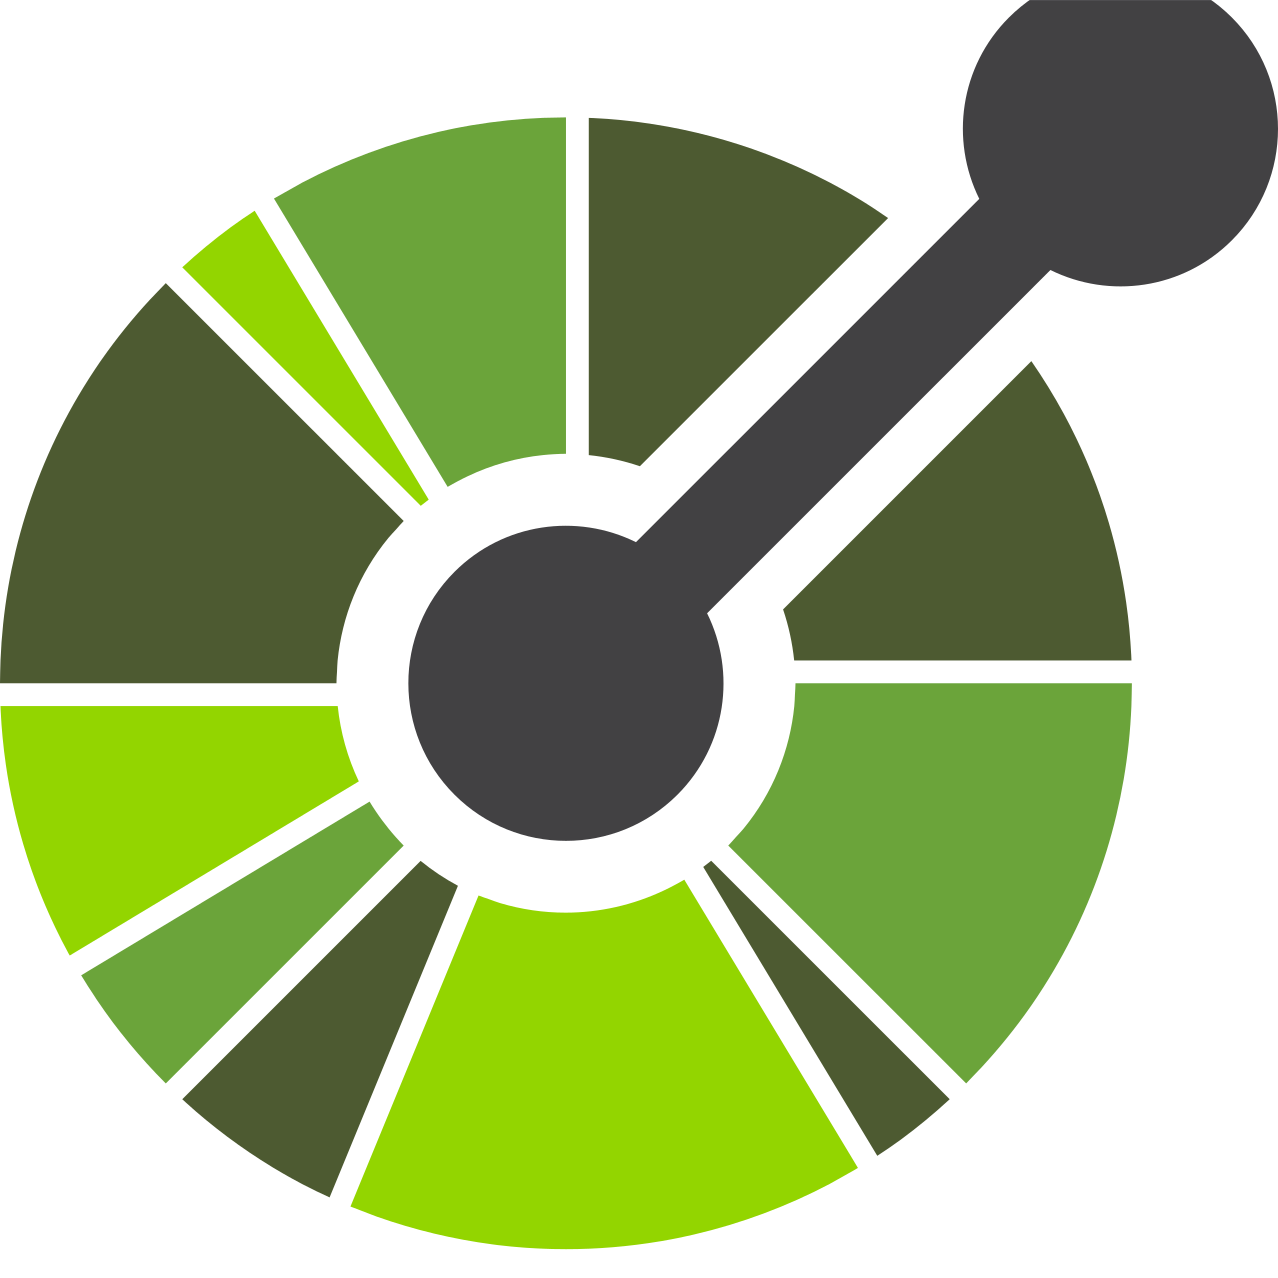
\includegraphics[width=0.8cm]{icons/openapi.pdf}};
        \node[
          text=bg-restapi, 
          anchor=west, 
          right=-3.8pt,
          font=\bfseries] at (restapi-icon.east) {dserver (OpenAPI-compliant REST API)};
  \end{pgfonlayer}
  \end{scope}
\end{tikzpicture}
}
\end{document}